\chapter{T\'ecnicas y herramientas de desarrollo}
\newpage

\section{Modelo de desarrollo}

Se ha decidido usar el modelo de desarrollo RUP (Rational Unified Process) para la implementaci\'on de este proyecto. RUP es un modelo que promueve el desarrollo iterativo y organiza la elaboraci\'on de software en 4 fases (inicio, elaboraci\'on, desarrollo y cierre) las cuales consisten de una o m\'as iteraciones ejecutables de este. 

\begin{figure}[H]
  \centering
  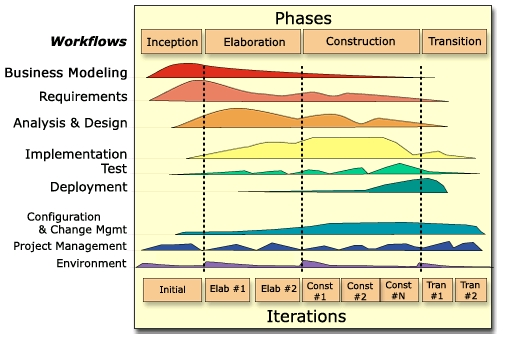
\includegraphics[scale=0.7]{Modelo.jpg}
  \caption[~RUP]{Diagrama del modelo RUP.}
  \label{fig:RUP}
\end{figure}

Este proyecto se separar\'a en cuatro secciones correspondientes a cada una de las entregas de ejecutables, las cuales se profundizar\'an en las cuatro iteraciones del ciclo de desarrollo. Las secciones son:

\begin{enumerate}
\item Funcionamiento b\'asico, dise\~no de robot
\item Implementaci\'on mascota virtual
\item Interacci\'on con robot
\item Interface, fluidez de interacci\'on entre mascota virtual y robot.
\end{enumerate}

De esta forma, se llevar\'an a cabo las distintas etapas de una manera iterativa, secuencial, modularizada e incremental.

Las especificaciones de los casos de uso y requerimientos se encuentran en el archivo ``Anexo.xlsx''.

\newpage
\section{Herramientas y t\'ecnicas de soporte para el de\-sa\-rro\-llo}

Para el desarrollo de Viper, el equipo Phyrex ha decidido utilizar las siguientes herramientas:

\begin{itemize}
    \item {\bf Sistema operativo Android 2.1 o superior}: Plataforma oficial de la aplicaci\'on
    \item {\bf Java}: Lenguaje de programaci\'on usado para la aplicaci\'on de Android
    \item {\bf C}: Lenguaje de programaci\'on usado para programar robot LEGO Mindstorms NXT
    \item {\bf UML}: Lenguaje de modelado de base de datos
    \item {\bf Photoshop }: Herramienta de dise\~no gr\'afico
    \item {\bf LEGO Digital Designer}: Herramienta de dise\~no y armado de estructuras de LEGO
    \item {\bf Google docs}: Herramienta de edici\'on colaborativa de documentos
    \item {\bf Git}: Herramienta de control de versiones
    \item {\bf Android SDK tools}: Herramientas de desarrollo en Android
    \item {\bf Eclipse}: Entorno de desarrollo para Android
    \item {\bf SQLite}: Base de datos para la aplicaci\'on
    \item {\bf LEGO Mindstorms NXT}: Robot programable de LEGO
    \item {\bf LEGO Mindstorms 2.0}: Ambiente de desarrollo para Mindstorms
    \item {\bf ROBOTC for LEGO Mindstorms}: Ambiente de desarrollo para Mindstorms
    \item {\bf Skype}: Herramienta de comunicaci\'on entre miembros del equipo
    \item {\bf Facebook}: Herramienta para comunicaci\'on de noticias del proyecto
    \item {\bf \LaTeX}: Edici\'on de documentos
    \item {\bf Microsoft Project}: Herramienta de creaci\'on y manejo de carta gantt
    \item {\bf StarUML}: Herramienta de modelado de casos de uso
    \item {\bf Trello}: Herramienta de gesti\'on de proyectos
\end{itemize}

\newpage
\section{Personal y capacitaci\'on del equipo de desarrollo}

Para el desarrollo del proyecto, se necesita contar con un equipo que tenga conocimientos en Java para desarrollo en Android, SQLite, ROBOTC para LEGO Mindstorms, y Photoshop. 

El equipo de desarrollo para este proyecto es la pre-empresa Phyrex, una pre-empresa formada por cuatro estudiantes de ingenier\'ia civil inform\'atica de la UTFSM, los cuales se presentan a continuaci\'on:

\begin{itemize}
\item {\bf Juan Avalo}: Experiencia en los lenguajes relevantes (Java, C). 
\item {\bf Celeste Bertin}: Experiencia previa en desarrollo en Android, aprendizaje r\'apido para resolver problemas nuevos. 
\item {\bf Roc\'io Fern\'andez}: H\'abil dise\~nadora gr\'afica, experiencia previa en desarrollo en Android, C y librer\'ia gr\'afica AndEngine. Uso avanzado de LEGO. 
\item {\bf Rodrigo Fr\'ias}: Experiencia en maquetaci\'on de textos y programaci\'on en C.
%\item {\bf Patricio Carrasco}: Programador con experiencia en varios lenguajes.
\end{itemize}

El equipo esta en constante aprendizaje de Android para sacarle el mayor provecho a esta tecnolog\'ia. El equipo esta en capacitaci\'on de ROBOTC a trav\'es de tutoriales y documentaci\'on disponible en la web. 
